\section{Introduction}

\begin{frame}
  \frametitle{Bibliographie}
  \begin{itemize}
    \item Ce cours est très largement inspiré de celui de Cyril \textsc{Gruau} : Conception d'une base de
      données, \url{http://cyril-gruau.developpez.com/merise/}
    \item Il est également inspiré par les cours réalisés par des enseignants de
      l'ENSEIRB-MATMECA:\\A. Zemmari, M. Mosbah, B. Le Saëc
    \item Outil de réalisation de diagrammes entité-association : \url{http://www.analysesi.com/}
  \end{itemize}
\end{frame}

\begin{framentitle}{Correctifs}
    \begin{itemize}
        \item Ce cours est disponible sous licence libre sur ce dépôt github:\\
            \small{\url{https://github.com/sfourestier/enseignement}}
        \item[$\ra$] Voici pouvez :
            \begin{itemize}
                \item L'améliorer en proposant des \emph{Pull requests}
                \item Partager autour de points pouvant être améliorés en créant des
                    tickets (\emph{Issues})
            \end{itemize}
    \end{itemize}
\end{framentitle}

\begin{frame}
  \frametitle{Historique}
  \begin{itemize}
    \item Informatique :\\
      Construire des systèmes pour effectuer des calculs (équations différentielles, calcul matriciel, etc.)
    \item Aujourd'hui, on s'appuie de plus en plus sur des données $\ra$ gestion de grandes quantités d'informations:
      \begin{itemize}
        \item Stocker des données
        \item Manipuler ces données
      \end{itemize}
    \item Données de natures diverses, opérations plus ou moins compliquées
    \item[$\ra$] On se place donc dans le cas des systèmes d'informations de gestion
        \begin{itemize}
            \item Manipulent beaucoup de données
            \item[$\ra$] Modélisation de la manière dont les données seront
                organisées
        \end{itemize}
  \end{itemize}
\end{frame}

\begin{frame}
  \frametitle{Objectif d'un SGBD}
  \begin{itemize}
    \item Stocker, centraliser des données (BD) et les mettre à disposition des utilisateurs
    \item Manipuler (de manière transparente pour l'utilisateur) des données (SGBD)
    \item Exemples d'utilisation :
      \begin{itemize}
        \item Gestion : paye, stock, etc.
        \item Transactionnelles : banque, réservation, etc.
        \item Documentation : bibliothèque, cartographie, etc.
      \end{itemize}
  \end{itemize}
\end{frame}

\begin{frame}
  \frametitle{Fonctionnalités d'un SGBD (1)}
  \begin{itemize}
    \item Gestion du stockage :\\
      Tailles importantes des données, éviter les redondances
    \item Persistance :\\
      Les données survivent aux programmes qui les créent
    \item Fiabilité :\\
      Mécanismes de reprise sur pannes (logiciel ou matériel)
    \item Sécurité/Confidentialité :\\
      Contrôle des utilisateurs et des droits d'accès aux données
    \item Interfaces homme-machine :\\
      Ergonomie, profils utilisateurs
    \item Distribution :\\
      Données stockées sur différents sites
    \item Optimisation
  \end{itemize}
\end{frame}

\begin{frame}
\frametitle{Fonctionnalités d'un SGBD (2)}
\begin{itemize}
  \item Contrôle de concurrence : propriétés ACID, transactions
    \begin{itemize}
      \item Atomicité :\\
        Soit toutes les opérations de la transaction sont validées, soit aucune ne l'est
      \item Cohérence :\\
        Préservation de la cohérence de la base (contraintes d'intégrité, etc.)
      \item Isolation :\\
        Quelle que soit la manière dont les transactions concurrentes sont exécutées, on doit pouvoir les
        ordonner de sorte à ce que l'état final de la base soit le même qu'après une exécution séquentielle
        des différentes transactions.
    \item Durabilité :\\
      Si une transaction est validée, tous les changements qu'elle a effectués sur la base sont persistants
    \end{itemize}
\end{itemize}
\end{frame}

\begin{frame}
  \frametitle{Architecture fonctionnelle d'un SGBD}
  \begin{center}
    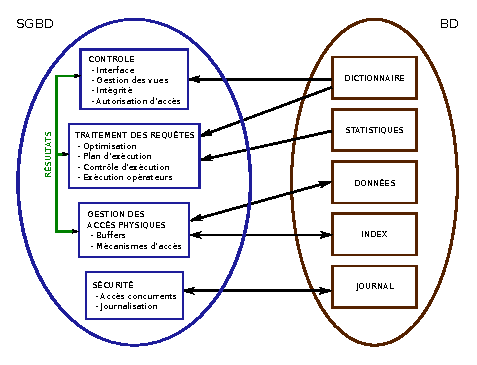
\epsfig{file=sgbd.eps,width=0.9\linewidth}
  \end{center}
\end{frame}

\begin{frame}
  \frametitle{Utilisateurs d'un SGBD}
  \begin{itemize}
    \item Administrateur
      \begin{itemize}
        \item Définition du schéma logique
        \item Définition des structures de stockage et les méthodes d'accès
        \item Gestion des autorisations
        \item Spécification des contraintes
        \item Maintenance de la performance
      \end{itemize}
    \item Concepteur et programmeur
      \begin{itemize}
        \item Est informaticien
        \item Connaît au moins le LMD
        \item Connaît bien le SGBD
        \item Connaît un ou plusieurs langages de programmation
      \end{itemize}
    \item Utilisateur
      \begin{itemize}
        \item Intervient en amont de la réalisation du SGBD
        \item Peut participer à la validation du schéma conceptuel
        \item Secrétariat, caissier, etc.
      \end{itemize}
  \end{itemize}
\end{frame}

\begin{frame}
  \frametitle{Niveau d'abstraction des données}
  \begin{center}
    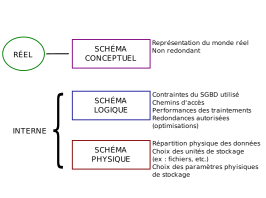
\includegraphics[width=\linewidth]{abstractions.pdf}
  \end{center}
\end{frame}

% \begin{frame}
%   \frametitle{Principes de base}
%   \begin{itemize}
%     \item Indépendance physique
%       \begin{itemize}
%         \item Les applications manipulant la base au niveau logique ne doivent pas être réécrites si la
%           structure physique est modifiée
%       \end{itemize}
%     \item Indépendance logique
%       \begin{itemize}
%         \item Une modification au niveau logique n'implique aucune modification des applications utilisant le
%           niveau externe
%       \end{itemize}
%     \item[$\ra$] Deux types de langages :
%       \begin{itemize}
%         \item Description des données (schéma)
%         \item Manipulation des données (instance) : requêtes et mise à jour
%       \end{itemize}
%   \end{itemize}
% \end{frame}

% \begin{frame}
%   \frametitle{Schéma et instance}
%   \begin{itemize}
%     \item Analogues à la notion de variable et de type dans les langages de programmation
%     \item Schéma : structure logique de la base de données
%       \begin{itemize}
%         \item Exemple : ensembles de clients, de produits et de fournisseurs
%       \end{itemize}
%     \item Instance : le contenu effectif de la base de données à un instant donné
%   \end{itemize}
% \end{frame}

\begin{frame}
  \frametitle{Modèles de données}
    On utilise la méthode MERISE :
  \begin{itemize}
    % \item Ensemble d'outils permettant de définir :
    %   \begin{itemize}
    %     \item Le schéma et les instances
    %     \item Les opérations possibles sur les instances
    %   \end{itemize}
    \item Modèle conceptuel de données :
      \begin{itemize}
        \item Entité-association
        \item (Diagramme de classes UML)
      \end{itemize}
    \item Modèle logique de données :
      \begin{itemize}
        \item Modèle relationnel
      \end{itemize}
    \item Modèle physique de données :
      \begin{itemize}
        \item Implémentation particulière du modèle logique de données par le logiciel
      \end{itemize}
  \end{itemize}
\end{frame}

\begin{frame}
  \frametitle{Conception d'une base de données}
  \begin{itemize}
    \item Conception d'une base de données:
      \begin{enumerate}
        \item Analyse des besoins
        \item Description conceptuelle
        \item Conception logique
        \item Conception physique
      \end{enumerate}
    \item Les 2 premières phases sont indépendantes du SGBD
    \item Le passage de 2 à 3 peut être en partie automatisé
  \end{itemize}
\end{frame}
